% Chapter 2: Flow Chart
% Financial Reporting Processes and Workflows

\chapter{Flow Chart}

\section{Financial Reporting Process Flow}

\subsection{Monthly Reporting Cycle}
The financial reporting process at Asia Trade \& Technology follows a monthly cycle. Field accountants collect financial data from project sites like Brahmanbaria. This data includes expenses for materials, labor, equipment, and other project costs.

The process has several stages: data collection, review, verification, approval, and payment processing. Each stage has specific responsibilities and timelines to maintain financial control.

\vspace{0.5em}
\begin{figure}[H]
    \centering
    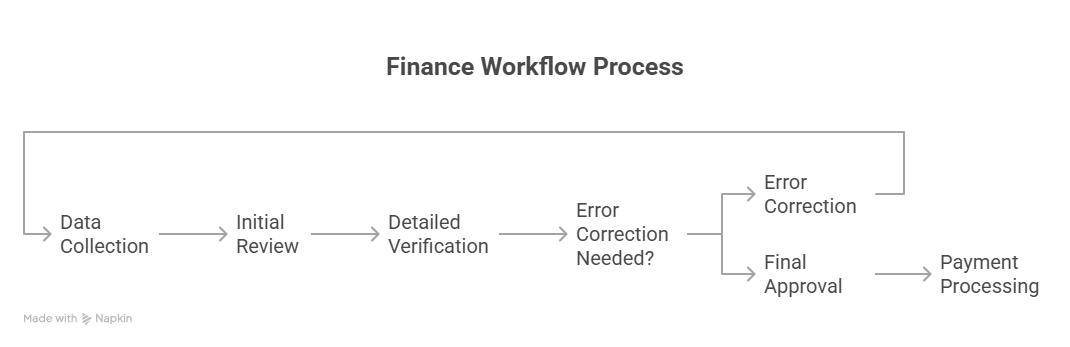
\includegraphics[width=0.9\textwidth]{assets/images/financial_flowchart.png}
    \caption{Monthly Financial Reporting Process Flow}
    \label{fig:financial_flowchart}
\end{figure}

Figure \ref{fig:financial_flowchart} shows the complete monthly financial reporting process flow from data collection to final payment processing.

\subsection{Key Process Stages}
The financial reporting process has five main stages:

1. **Data Collection**: Field accountants gather receipts, invoices, and other documents during the first week of each month.

2. **Initial Review**: The Dhaka office accounting team checks documents for completeness and basic accuracy.

3. **Detailed Verification**: Each expense is carefully examined for accuracy, budget compliance, and proper authorization.

4. **Error Correction**: If issues are found, reports are returned to field accountants for correction and resubmission.

5. **Final Approval**: After verification, the Dhaka manager approves the report and sends it to Beijing headquarters for payment processing.

\vspace{0.5em}
\section{Document Management System}

\subsection{Document Organization}
The company organizes financial documents into categories: receipts, invoices, timesheets, purchase orders, and project reports. Documents are stored by project, date, and expense type for easy access.

\begin{figure}[H]
    \centering
    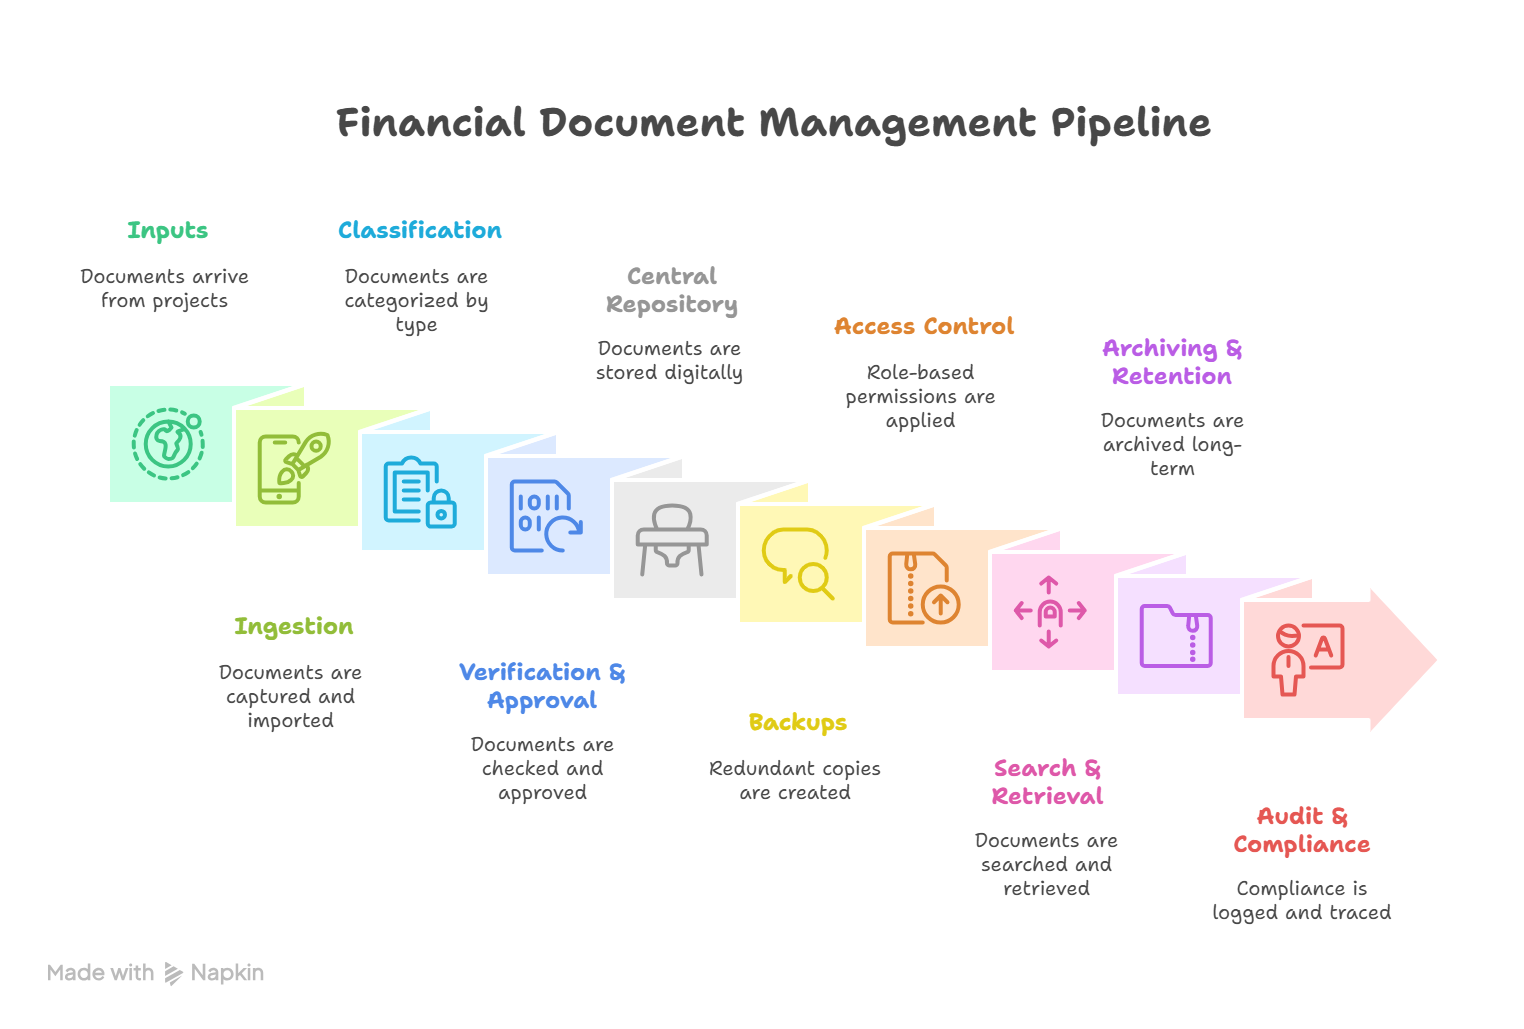
\includegraphics[width=0.9\textwidth]{assets/images/document_management.png}
    \caption{Document Management System Architecture}
    \label{fig:document_management}
\end{figure}

Figure \ref{fig:document_management} shows the document management system flow from input through classification, verification, storage, and archiving.

\subsection{Document Processing}
Receipts and invoices are the most important documents. Each document is checked for completeness, proper authorization, and accuracy. The company uses both digital and physical storage systems with backup procedures, access controls, and regular audits to ensure security and compliance with international standards.

\vspace{0.5em}
\section{Approval Hierarchy}

\subsection{Three-Level Approval System}
The company uses a three-level approval system for financial decisions:

1. **Field Level**: Field accountants in Brahmanbaria review and approve local expenses
2. **Office Level**: Dhaka office managers provide oversight and validate field decisions  
3. **Headquarters Level**: Beijing headquarters gives final approval and strategic oversight

\begin{figure}[H]
    \centering
    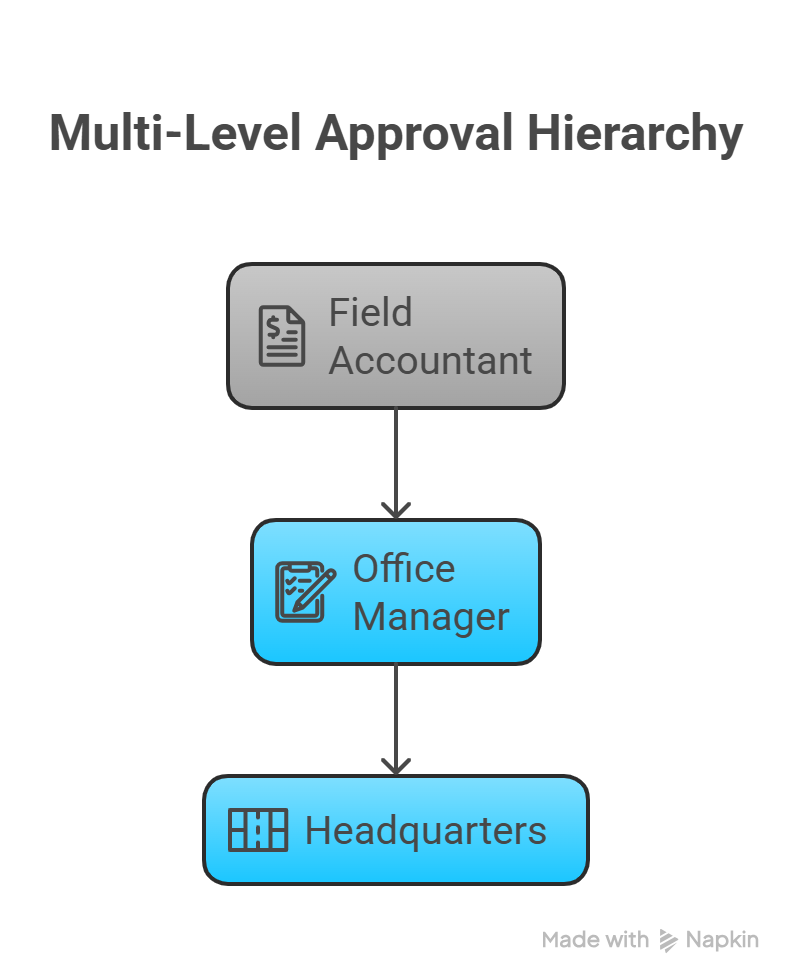
\includegraphics[width=0.9\textwidth]{assets/images/approval_hierarchy.png}
    \caption{Multi-Level Approval Hierarchy Structure}
    \label{fig:approval_hierarchy}
\end{figure}

Figure \ref{fig:approval_hierarchy} shows the three main levels of authority and their responsibilities.

\subsection{Key Responsibilities}
- **Field Accountant**: Reviews expenses, checks documentation, prepares monthly reports
- **Office Manager**: Reviews calculations, verifies budget limits, ensures policy compliance
- **Headquarters**: Final budget review, corporate standards, regulatory compliance

The system ensures proper oversight while maintaining efficient operations.

\vspace{0.5em}
\section{Budget Control}

\subsection{Budget Management}
The company plans project budgets based on requirements, technical specs, and market conditions. Budgets are allocated across different project activities and categories. The process is regularly reviewed and updated as project needs change.

\begin{figure}[H]
    \centering
    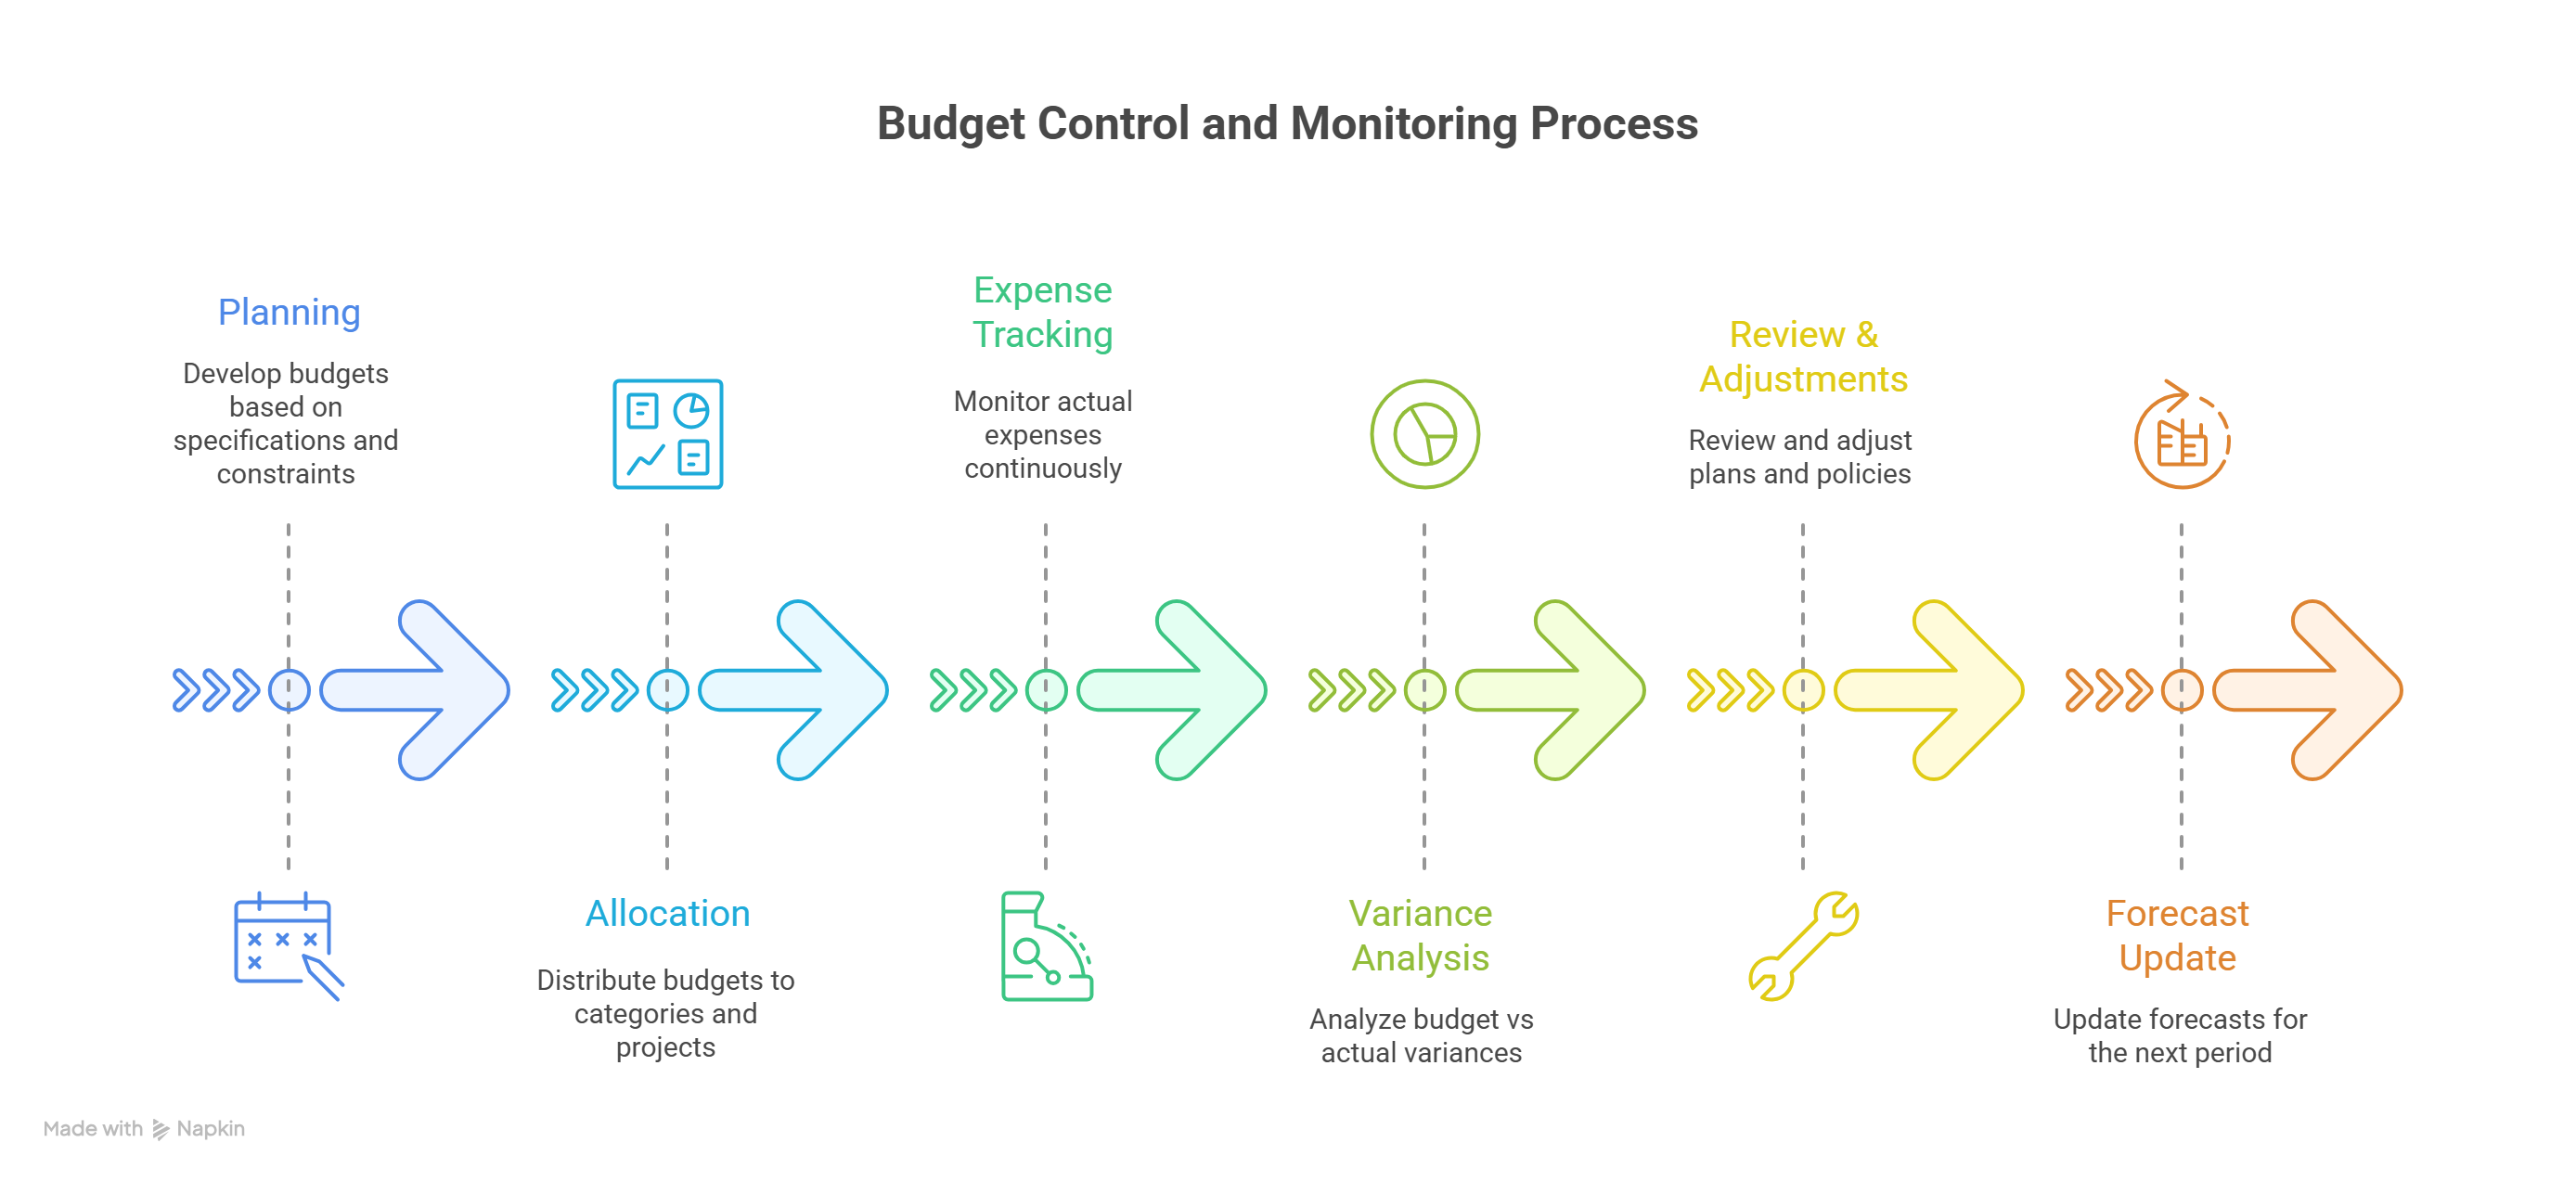
\includegraphics[width=0.9\textwidth]{assets/images/budget_control.png}
    \caption{Budget Control and Monitoring Process}
    \label{fig:budget_control}
\end{figure}

Figure \ref{fig:budget_control} shows the budget control process from planning through monitoring and evaluation.

\subsection{Budget Monitoring and Control}
The company monitors expenses in real-time against budgeted amounts, tracks expense trends, and analyzes variances between budgeted and actual expenses. Regular reviews help identify cost issues early and determine if corrective action is needed. Budget adjustments are allowed when project requirements change, but must be properly documented and authorized.
